\documentclass[12pt]{article}

\usepackage[top=1in, bottom=1in, left=1in, right=1in]{geometry}
\usepackage[T1]{fontenc}
\usepackage{mathptmx}
\usepackage{amsmath, amssymb, amsthm}
\usepackage{enumitem}
\usepackage{booktabs}
\usepackage{graphicx}
\usepackage{setspace}
\usepackage{xcolor}
\usepackage[colorlinks=true, linkcolor=blue, citecolor=blue, urlcolor=blue]{hyperref}

% Drafting annotations — coloured inline comments. Requires xcolor (loaded above).
\newcommand{\ignacio}[1]{\textcolor{blue}{#1}}
\newcommand{\michael}[1]{\textcolor{red}{#1}}

\linespread{1.15}

\title{The effects of AI recommendation on epistemic diversity}
\author{}
\date{}

\begin{document}
\maketitle

I describe a simple model (sections~\ref{sec:bandit}--\ref{sec:airec}), make some guesses about how the model may behave (section~\ref{sec:conj}), and discuss some potentially philosophically interesting consequences of these conjectures (sections~\ref{sec:improve}--\ref{sec:mech}). The model comes with a small Python implementation, which I outline before turning to the model itself.

\section*{Implementation}

The model is realised as a small, self-contained Python package, \texttt{model/}, with one module per modelling primitive. \texttt{BernoulliBandit} holds the two arms and their Bernoulli means and enforces $p_A > p_B$. \texttt{BetaBernoulliAgent} is a single agent: it keeps one Beta posterior per arm, chooses by posterior mean, and performs the conjugate update on each observed payoff. \texttt{Recommender} is the interface for the AI of sections~\ref{sec:airec}--\ref{sec:improve}; \texttt{NullRecommender} abstains (the unaided regime), and the two Phase 2 operationalisations of section~\ref{sec:airec} are \texttt{EvidenceSharingRecommender} and \texttt{ChoiceNudgeRecommender}. \texttt{discovery.py} collects the operational definitions of the discovery event $D_i$ (section~\ref{sec:bandit}), and \texttt{run\_simulation} is the orchestrator.

The simulation is a single loop. A community of $n$ agents faces the shared bandit for $T$ stages; at each stage every agent (i)~optionally receives a recommendation, (ii)~pulls the arm with the higher posterior expected payoff, (iii)~observes a Bernoulli payoff, and (iv)~updates the posterior of the pulled arm. Each agent draws from its own random stream, spawned from one master seed via \texttt{SeedSequence.spawn}, so the agents are statistically independent yet the run as a whole is reproducible. The accompanying notebooks reproduce the unaided results of section~\ref{sec:unaided}; the recommenders of section~\ref{sec:airec} are implemented and unit-tested, with their dedicated experiment notebook still to come.

\section{Standard two-armed bandit}
\label{sec:bandit}

Start with a standard two-armed bandit model.
There are two arms, $A$ and $B$.
Arm $A$ has mean payoff $p_A$.
Arm $B$ has mean payoff $p_B$.
Assume $p_A > p_B$, so $A$ is the better arm.
We take the payoffs to be Bernoulli: pulling an arm returns $1$ with probability equal to that arm's mean and $0$ otherwise. This is the natural choice here, because Bernoulli payoffs are conjugate to the Beta beliefs the agents carry below, so each observation updates a belief in closed form.

There are $n$ agents.
Assume for now that agents do not communicate or observe others' payoffs.
Each agent carries two independent Beta beliefs, one over $p_A$ and one over $p_B$; unless stated otherwise these start uniform, $\mathrm{Beta}(1,1)$, and the same prior is shared across the community. Because the payoffs are Bernoulli, an agent conditions on an observed payoff by the conjugate update: a success increments that arm's $\alpha$, a failure its $\beta$. Each agent conditions only on its own payoffs.

Every agent is a myopic Bayesian.
At every stage it pulls the arm with the higher posterior expected payoff, that is, the arm with the larger posterior mean $\alpha_i/(\alpha_i + \beta_i)$, breaking ties uniformly at random.

Let $D_i$ be the event that agent $i$ discovers which is the better arm. We make this precise through two operational criteria, both evaluated on the agent's state at the end of the run and both implemented in \texttt{discovery.py}:
\begin{enumerate}[leftmargin=*]
  \item \emph{Last-$k$}: the agent's last $k$ pulls are all of arm $A$, so it has, in effect, settled on the better arm.
  \item \emph{Posterior gap}: the agent's posterior means separate in the right direction by at least a margin $\delta$, that is $E[p_A \mid h] - E[p_B \mid h] \geq \delta$.
\end{enumerate}
The two criteria need not agree on any single run, but they coincide with high probability once the horizon is long: an agent that has pulled $A$ for many consecutive steps has typically also built up a posterior-mean gap in $A$'s favour, and conversely. We therefore treat $D_i$ as well defined up to this asymptotic equivalence and report results under both criteria.

The community succeeds ($D$) if at least one agent succeeds, so
\[
  D = D_1 \cup \cdots \cup D_n.
\]

\section{Unaided collective success}
\label{sec:unaided}

I use $P$ for the ``objective'' probabilities determined by the model specifications. Write $q = P(D_i)$ for the individual discovery probability, which by symmetry is the same for every agent.

\paragraph{What fixes $q$.}
Under this objective reading $q$ is not a free parameter; it is fixed by the gap between the arms, the prior, the discovery criterion, and in principle the horizon. The gap is the primary driver. Writing $\Delta = p_A - p_B$, when $\Delta$ is large the arms are easy to tell apart and $q$ is high, whereas as $\Delta \to 0$ they become statistically indistinguishable and $q$ falls toward the level a non-discovering agent would reach by chance. We measure discovery by the posterior-gap criterion of section~\ref{sec:bandit}, with the margin scaled to the problem as $\delta = \Delta/2$: strictly below the true gap, so that an agent whose posterior means have converged near the truth clears it, whereas a margin above $\Delta$ would be unreachable even for a perfectly informed agent. Under the flat prior adopted throughout, the horizon turns out to drop out: $q$ reaches its long-run value well before $T = 1000$ and stays there (as the simulation below verifies), so the values we report are equilibrium properties of the model rather than finite-horizon readings. Rather than postulate a value for $q$, then, we read it off the model for a given gap.

\paragraph{The prior.}
It is worth being explicit about how the simulation initialises the beliefs, since the prior sets each agent's starting point and its early inertia. Every agent begins each arm at a uniform $\mathrm{Beta}(1,1)$ belief, and all $n$ agents in a community are given the same prior. A $\mathrm{Beta}(1,1)$ is flat on $[0,1]$: it expresses no preference between the arms, so both posterior means start at $\tfrac12$ and the first pull is a coin flip, and it lets the earliest observations move a belief a long way, since after $a$ successes and $b$ failures on an arm the posterior mean is $(a+1)/(a+b+2)$. A more concentrated prior $\mathrm{Beta}(\alpha_0,\beta_0)$ with larger $\alpha_0+\beta_0$ would damp those early swings and make an agent harder to divert from a good arm; an asymmetric prior would bias which arm an agent favours before seeing any data. We keep the flat, shared prior as the baseline, and not merely for neutrality: it is also what makes $q$ stationary. A concentrated prior $\mathrm{Beta}(s,s)$ contributes $2s$ pseudo-observations pinning both posterior means at $\tfrac12$, so beliefs cannot separate until the accumulated evidence outweighs them ($T \gg 2s$), and any $q$ measured at a horizon comparable to $s$ is a finite-horizon transient still climbing toward its long-run value (notebook 1c documents this directly: at $s = 800$, $\hat q_{\text{gap}}$ runs $0.003 \to 0.39$ as $T$ goes $1000 \to 8000$). Under the flat prior, by contrast, beliefs converge well within $T = 1000$ and the measured $q$ does not move thereafter.

\paragraph{An analytic handle as $T \to \infty$.}
The myopic rule never explores for its own sake; it always pulls the arm it currently believes is better, and this makes the long-run behaviour tractable. If both arms were pulled infinitely often, their posterior means would converge to $p_A$ and $p_B$; since $p_A > p_B$ the agent would then prefer $A$ from some point on, contradicting infinitely many $B$-pulls. So each agent pulls one arm only finitely often and the other forever: the play \emph{absorbs} on a single arm. In this limit the last-$k$ criterion becomes exactly the event that the agent absorbs on $A$, and the posterior-gap criterion becomes that same event together with the mild condition that the final gap clears $\delta$; to leading order both give
\[
  q \;=\; P(\text{the agent settles on } A).
\]
This probability lies strictly between $0$ and $1$. It is below $1$ because of \emph{incomplete learning}: an unlucky early run on $A$ can pull its posterior mean below that of $B$, so the agent switches to $B$; if by then $A$'s mean has fallen below $p_B$, then once $B$'s posterior mean settles near $p_B$ it stays above $A$'s frozen value forever, and the agent never samples $A$ again or collects the evidence that would correct it. It is above $0$ because a good early run locks the agent onto $A$ in the same way. There is no elementary closed form at general $(p_A, p_B)$: writing $f(\alpha_A, \beta_A, \alpha_B, \beta_B)$ for the probability of eventually settling on $A$ from a given pair of Beta states, $q = f(\alpha_0, \beta_0, \alpha_0, \beta_0)$ solves a fixed-point recursion over those states, which the Phase 1 simulation evaluates by Monte Carlo rather than in closed form. What is clear analytically is the shape: $q$ increases with the gap $\Delta$, it stays strictly below $1$ for every finite gap while approaching $1$ as the gap widens, and the prior enters only through the common starting state. This ceiling below $1$ is what makes the community question non-trivial; if individuals discovered $A$ almost surely there would be nothing for the AI to spoil.

\paragraph{Simulation: the stationary $q$.}
The notebook \texttt{experiments/1d.\ Phase 1 - Flat Prior.ipynb} makes this concrete. Centering the arms at $\tfrac12$ (so $p_A = \tfrac12 + \Delta/2$ and $p_B = \tfrac12 - \Delta/2$), it runs $n = 500$ independent agents per gap from the shared flat prior for $T = 10000$ steps and reads $\hat q_{\text{gap}}(t)$ off the reconstructed posterior trajectories at every intermediate horizon, for the three studied gaps $\Delta \in \{0.01, 0.1, 0.5\}$ (Figure~\ref{fig:flatprior-qtraj}). Two findings. First, stationarity: over the window $t \in [1000, 10000]$ the drift in $\hat q_{\text{gap}}$ is inside two binomial standard errors at every gap, and the $t = 1000$ reading already equals the $t = 10000$ reading, so $T = 1000$ is comfortably inside equilibrium. Second, the stationary level rises with the gap but stays well short of $1$ even at $\Delta = 0.5$, where the arms ($p_A = 0.75$ against $p_B = 0.25$) are about as distinguishable as the setup allows: the incomplete-learning ceiling of the analytic-handle paragraph is visible at every gap.

\begin{center}
\small
\begin{tabular}{lcccc}
\toprule
\multicolumn{5}{c}{\textbf{Flat-prior gap sweep} \quad ($\mathrm{Beta}(1,1)$, posterior gap $\delta = \Delta/2$, $n = 500$ per gap; notebook 1d)}\\
\midrule
$\Delta$ & $\delta$ & $\hat q_{\text{gap}}(t = 10^3)$ & $\hat q_{\text{gap}}(t = 10^4)$ & drift over $[10^3, 10^4]$ \ (vs.\ $2\,\mathrm{SE}$)\\
\midrule
$0.01$ & $0.005$ & $0.492$ & $0.490$ & $0.004$ \ $(0.045)$\\
$0.10$ & $0.05$  & $0.636$ & $0.618$ & $0.022$ \ $(0.043)$\\
$0.50$ & $0.25$  & $0.824$ & $0.814$ & $0.030$ \ $(0.035)$\\
\bottomrule
\end{tabular}
\end{center}

\begin{figure}[t]
  \centering
  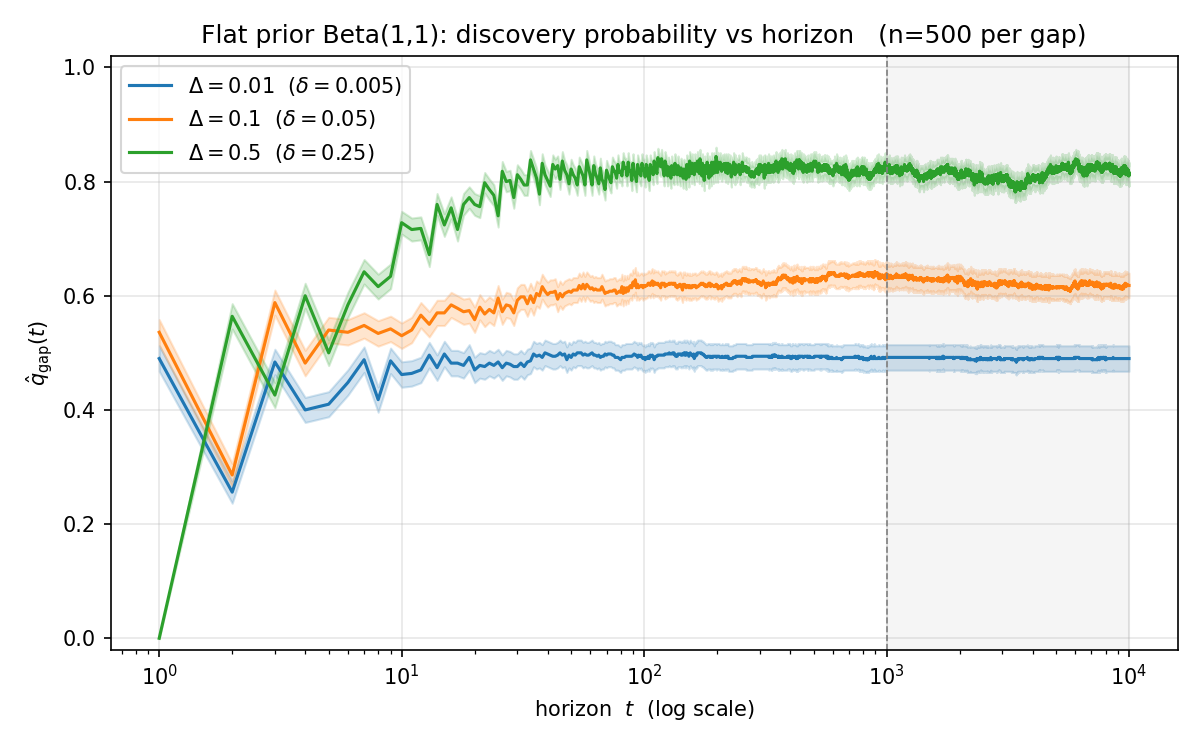
\includegraphics[width=0.85\textwidth]{../results/phase1_flat_prior_q_traj_20260610_161746.png}
  \caption{Discovery probability against the horizon under the flat prior: $\hat q_{\text{gap}}(t)$ for the three studied gaps $\Delta \in \{0.01, 0.1, 0.5\}$ with $\delta = \Delta/2$, $n = 500$ agents per gap (notebook 1d). Bands are $\pm 1$ binomial standard error; the horizontal axis is logarithmic; the shaded region marks the reporting window $t \in [10^3, 10^4]$. After an early transient, every curve is flat across the entire window: the $q$ values of the table are equilibrium properties, not finite-horizon readings.}
  \label{fig:flatprior-qtraj}
\end{figure}

\paragraph{The operating point: $\Delta = 0.01$.}
In what follows we focus on the smallest of the studied gaps, $\Delta = 0.01$, that is $p_A = 0.505$ and $p_B = 0.495$. This is the epistemically interesting regime: the two theories are nearly indistinguishable on the evidence, and the stationary discovery probability sits at $q \approx 0.49$ --- almost exactly a coin flip, the chance level predicted by the absorption argument. Individual discovery is genuinely contingent here, neither rare nor reliable, which leaves the recommender of section~\ref{sec:airec} the most room to move it in either direction; and because the value is stationary, whatever the recommender does to $q$ will be an effect on an equilibrium, not on a transient.

\paragraph{The community baseline.}
At the operating point $q \approx 0.49$, no individual agent is reliable, yet the community very much is. Because the agents are independent, with $n = 100$ agents,
\[
  P(D) = 1 - (1-q)^n = 1 - (1 - 0.49)^{100} = 1 - 0.51^{100} \approx 1 - 6 \times 10^{-30},
\]
indistinguishable from certainty: for the community to fail, one hundred independent near-coin-flips must all land on the worse arm. This is the unaided baseline, and it is what the simulation produces: the measured fraction of communities in which at least one agent discovers $A$ agrees with the closed form $1 - (1-\hat q)^n$, because with no recommender the agents share no common state and so remain genuinely independent.

\section{AI recommender}
\label{sec:airec}

Now introduce an AI recommender.
At each stage $t$, agent $i$ gives the recommender her private history $h_i^t$ (which arms she has pulled and which payoffs she has received).
By conditioning on that history, the agent also has posterior $\pi_i^t$.
The recommender $\rho$ takes these two things as inputs and returns a recommendation
\[
  R_i^t := \rho(h_i^t, \pi_i^t, Z) \in \{A, B\}.
\]

\ignacio{Interface implemented in \texttt{model/recommender.py}: abstract \texttt{Recommender.recommend(agent\_id, history, posterior\_alpha\_beta, rng)} returns an optional \texttt{Recommendation}. \texttt{NullRecommender} (always abstains) gives the unaided regime; the two operationalisations below are implemented as \texttt{EvidenceSharingRecommender} and \texttt{ChoiceNudgeRecommender}.}

The variable $Z$ represents the features of the recommender that are common among all agents, e.g.\ the algorithm that $\rho$ uses to make recommendations.
Suppose (here is a big simplification) $Z \in \{G, F\}$, that is, $Z$ can be in two states (a good state or a failure state).
Suppose
\[
  P(Z = G) = 0.99, \qquad P(Z = F) = 0.01.
\]

\ignacio{\textbf{Interpretive question about $Z$ --- now an implemented switch.} The paper writes $P(Z=G)=0.99$, which reads like an exogenous draw, while the prose says $Z$ ``represents the features of the recommender''. Two readings were on the table: (1) a \emph{per-community draw} of the recommender's hidden type, sampled once; (2) Michael's \emph{frequentist} reading, $G$/$F$ as the fraction of the time a single fixed recommender is well/poorly behaved, i.e.\ re-drawn independently across recommendations. The resolution is that we need not choose: both are implemented as the \texttt{z\_mode} switch (\texttt{'community'} draws $Z$ once per simulation; \texttt{'per\_share'} re-flips it on every recommendation), and they play different roles. Re-flipping makes the recommender's errors \emph{independent} across agents, so no common state is injected, the agents remain independent, and the community baseline $1-(1-q)^n$ survives --- reading (2) is the natural \emph{control condition}. The diversity mechanism of \S\ref{sec:mech} requires the common draw of reading (1). The realized $Z$ is recorded on \texttt{SimulationResult.z}, so $P(D \mid Z)$ can be reported empirically per trial.}

\michael{Interpretation 2 is what I had in mind originally.}


In the fully Bayesian protocol, every agent remains a myopic Bayesian but conditions on the AI recommendation before deciding which arm to pull: first the agent conditions on his history to get the posterior $\pi_i^t$, then he conditions on $R_i^t$, and finally he chooses the arm with the higher $\pi_i^t(\,\cdot \mid R_i^t)$ expected payoff. That protocol requires a likelihood $P(R \mid \text{better arm}, h, \pi, Z)$ and a stance on whether the agent knows $P(Z=G)$. We set it aside for now (the hook \texttt{apply\_recommendation} deliberately remains unimplemented) and instead study two operationalisations of $\rho$ that sidestep recommendation likelihoods altogether.

\michael{I hadn't thought about whether the agents know the value of $P(Z=G)$. Perhaps both options are worth investigating eventually? I don't know. I suggest we start with whether is simplest.}

\paragraph{Operationalisation 1: an evidence-sharing recommender.}
The recommender is a distinguished agent with a directed edge to every user: at each stage it pulls the \emph{true} bandit and shares the draw with each agent as a labeled observation, which the agent folds into the corresponding arm's posterior by the ordinary conjugate update (shared evidence moves beliefs but does not enter the agent's own pull history). Draws are i.i.d.\ across agents given $Z$, so the only common cause the recommender injects is $Z$ itself. The latent state acts on the data stream, in one of two variants (\texttt{EvidenceSharingRecommender}, \texttt{variant}):
\begin{enumerate}[leftmargin=*]
  \item \emph{State-selected source} (\texttt{state\_arm}): in $G$ the recommender samples and truthfully labels the better arm $A$; in $F$, the worse arm $B$. All labels are honest --- the failure state shares true data about the wrong theory.
  \item \emph{Confused labels} (\texttt{confused}): the recommender is a tutor sampling both arms in alternation; in $G$ its labels are correct, in $F$ the two theories' identities are swapped, so draws from $B$ are reported as evidence about $A$ and vice versa. Every agent's posterior gap is then driven toward $-\Delta$.
\end{enumerate}
The notebook \texttt{experiments/2.\ Phase 2 - Evidence Sharing.ipynb} studies this operationalisation in three steps: individual discovery by state at the \S\ref{sec:unaided} operating point, the horizon dependence of the confused variant, and the community-level effect. We report each in turn.

\paragraph{Operationalisation 2: a choice-nudging recommender.}
Here $R_i^t$ is (probabilistically) the agent's actual next pull, and Bayesian conditioning is abstracted away into a $Z$-dependent accuracy shift: in $G$ the recommender points at $A$, in $F$ at $B$, and the agent pulls the pointed arm with probability $\varepsilon$, choosing myopically otherwise (\texttt{ChoiceNudgeRecommender}, \texttt{follow\_prob}). No belief update on $R$ takes place; beliefs change only through the honest payoffs of whatever arm is pulled. So $G$ boosts arm $A$ a bit and $F$ boosts arm $B$, directly at the level of choice.

\paragraph{Results 1: individual discovery by state.}
At the \S\ref{sec:unaided} operating point ($\Delta = 0.01$, $\delta = 0.005$, flat prior, $T = 2000$; $n = 300$ agents per condition, $Z$ forced to each state via the prior over $Z$), the posterior-gap criterion gives the table below (Figure~\ref{fig:es-individual}). Both states of both variants move individual discovery in the intended direction. The striking entry is the honest variant's failure state: a recommender that only ever shares \emph{true} data --- merely about the wrong theory --- cuts individual discovery from $0.48$ to $0.14$. The mechanism is a comparison race: a trusted stream about one arm pins that arm's posterior at its true mean, so it never has misleading-looking stretches. Pinning $A$ (the $G$ state) cures the unaided model's characteristic failure, an unlucky early run freezing $A$'s posterior low, and lifts $q$ to $0.91$. Pinning $B$ (the $F$ state) removes the \emph{recovery channel}: unaided, an agent that wrongly switched to $B$ returns to $A$ when its own $B$-draws happen to look bad; with $B$'s posterior held at $p_B$ that escape disappears, and early dips of $A$'s posterior become permanent. The \texttt{per\_share} rows show each variant under independently re-flipped $Z$ at $P(Z = G) = 0.99$: close to the corresponding $G$ column, as expected of a $99\%$/$1\%$ mixture stream.

\begin{center}
\small
\begin{tabular}{lcc}
\toprule
\multicolumn{3}{c}{\textbf{Evidence sharing, individual level} \quad ($\Delta = 0.01$, $\delta = 0.005$, $T = 2000$, $n = 300$; notebook 2)}\\
\midrule
condition & $\hat q_{\text{gap}}$ & se\\
\midrule
unaided (\S\ref{sec:unaided} baseline) & $0.480$ & $0.029$\\
\texttt{state\_arm}, $Z = G$ & $0.910$ & $0.017$\\
\texttt{state\_arm}, $Z = F$ & $0.140$ & $0.020$\\
\texttt{confused}, $Z = G$ & $0.643$ & $0.028$\\
\texttt{confused}, $Z = F$ & $0.373$ & $0.028$\\
\texttt{state\_arm}, per-share mix & $0.850$ & $0.021$\\
\texttt{confused}, per-share mix & $0.657$ & $0.027$\\
\bottomrule
\end{tabular}
\end{center}

\begin{figure}[t]
  \centering
  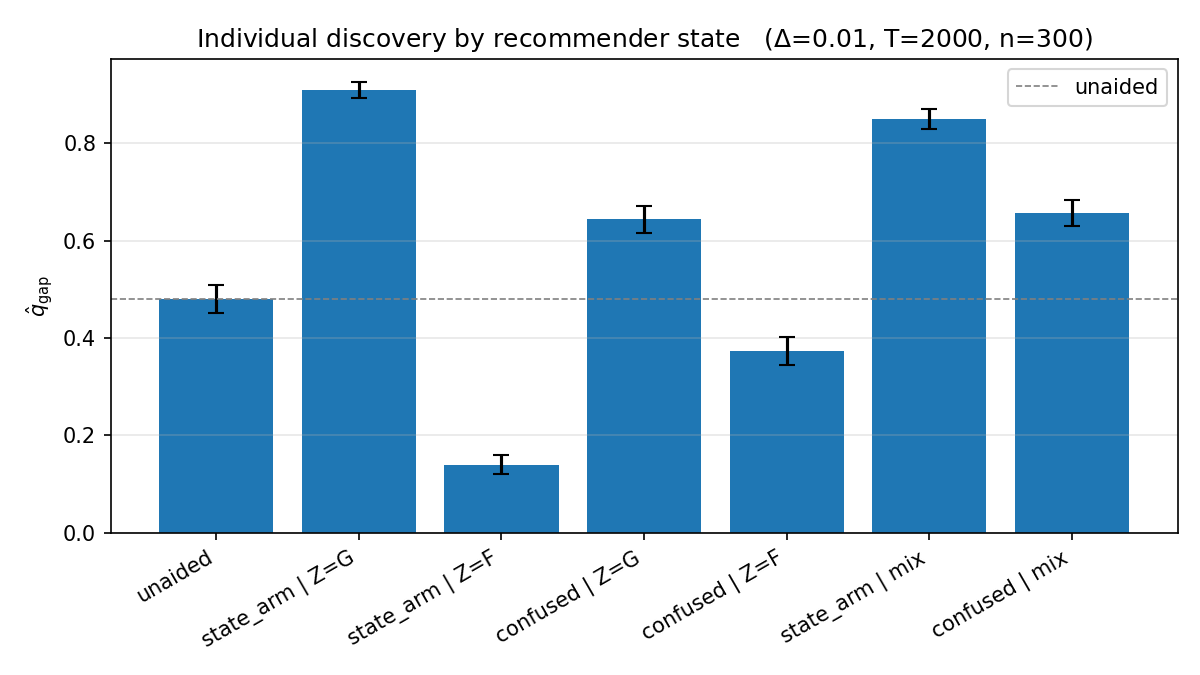
\includegraphics[width=0.75\textwidth]{../results/phase2_es_individual_20260610_174604.png}
  \caption{Individual discovery probability by recommender state for the evidence-sharing recommender ($\Delta = 0.01$, $\delta = 0.005$, $T = 2000$, $n = 300$ agents per condition; notebook 2). Bars are $\hat q_{\text{gap}}$ with $\pm 1$ binomial-SE error bars; the dashed line is the unaided baseline.}
  \label{fig:es-individual}
\end{figure}

\paragraph{Results 2: the confused variant separates on horizons $T \gtrsim 1/\Delta^2$.}
The confused failure state drives \emph{every} agent's posterior gap toward $-\Delta$, so $q_F \to 0$ and $q_G \to 1$ --- but only once the shared stream's own sampling noise falls below the criterion margin. After $T$ steps each arm has received about $T/2$ shared draws, so the pinned posterior means still fluctuate by $\sim \sqrt{1/(2T)}$, and separation requires this to be small against $\delta = \Delta/2$, i.e.\ $T \gtrsim 1/\Delta^2$. At $\Delta = 0.01$ that is $10^4$--$10^5$ steps, and the sweep confirms it (Figure~\ref{fig:es-horizon}): $\hat q_G$ climbs $0.65 \to 0.87$ and $\hat q_F$ falls $0.42 \to 0.11$ as $T$ goes $10^3 \to 3 \times 10^4$, heading to $1$ and $0$ but visibly incomplete even at $T = 30000$. This is purely a speed limit, not a structural one, which is why the community demonstration below moves to a coarser gap.

\begin{figure}[t]
  \centering
  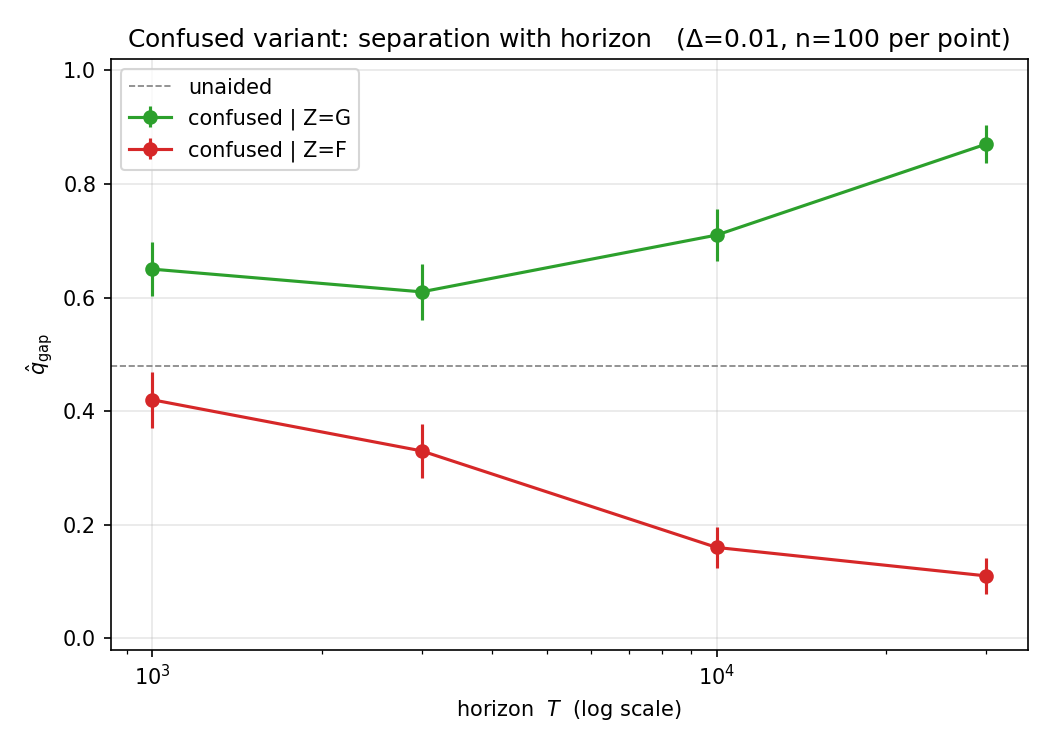
\includegraphics[width=0.7\textwidth]{../results/phase2_es_horizon_20260610_174604.png}
  \caption{Horizon dependence of the confused variant at the operating point $\Delta = 0.01$ ($n = 100$ agents per point, $Z$ forced; notebook 2). The good state climbs toward $1$ and the failure state falls toward $0$ on the $T \gtrsim 1/\Delta^2$ timescale set by the shared stream's sampling noise.}
  \label{fig:es-horizon}
\end{figure}

\paragraph{Results 3: individuals improve, the community gets worse.}
At $\Delta = 0.1$, $\delta = 0.05$, $T = 3000$ the confused variant's separation is complete --- measured $q_G = 1.000$, $q_F = 0.000$, against an unaided $q_u = 0.650$ --- so the \S\ref{sec:improve} effect can be exhibited with measured quantities (Figure~\ref{fig:es-community}). Given $Z$ the agents are i.i.d.\ (shared draws are independent per agent), so community discovery obeys the exact closed form $P(D \mid Z) = 1 - (1 - q_Z)^n$, verified in the notebook by bootstrap resampling of communities from the per-agent outcomes. Every individual improves: $P(D_i) = 0.99 \times 1.000 + 0.01 \times 0.000 = 0.990 \gg 0.650$. The community nonetheless deteriorates: unaided, $P(D) = 1 - 0.35^{100} \approx 1$; aided with a common $Z$, $P(D) = 0.99 \times 1 + 0.01 \times 0 = 0.990$. The aided community fails exactly when the shared recommender is in its failure state, and this $0.01$ failure mass cannot be diversified away --- the $P(D)$-versus-$n$ curve plateaus at $P(Z = G)$ instead of approaching $1$. The control isolates the mechanism: the \texttt{per\_share} recommender, with an identical marginal data stream but $Z$ re-flipped on every share, restores $P(D) \approx 1$. The harm is attributable entirely to the \emph{commonness} of $Z$, not to the recommender's $1\%$ error rate.

\begin{figure}[t]
  \centering
  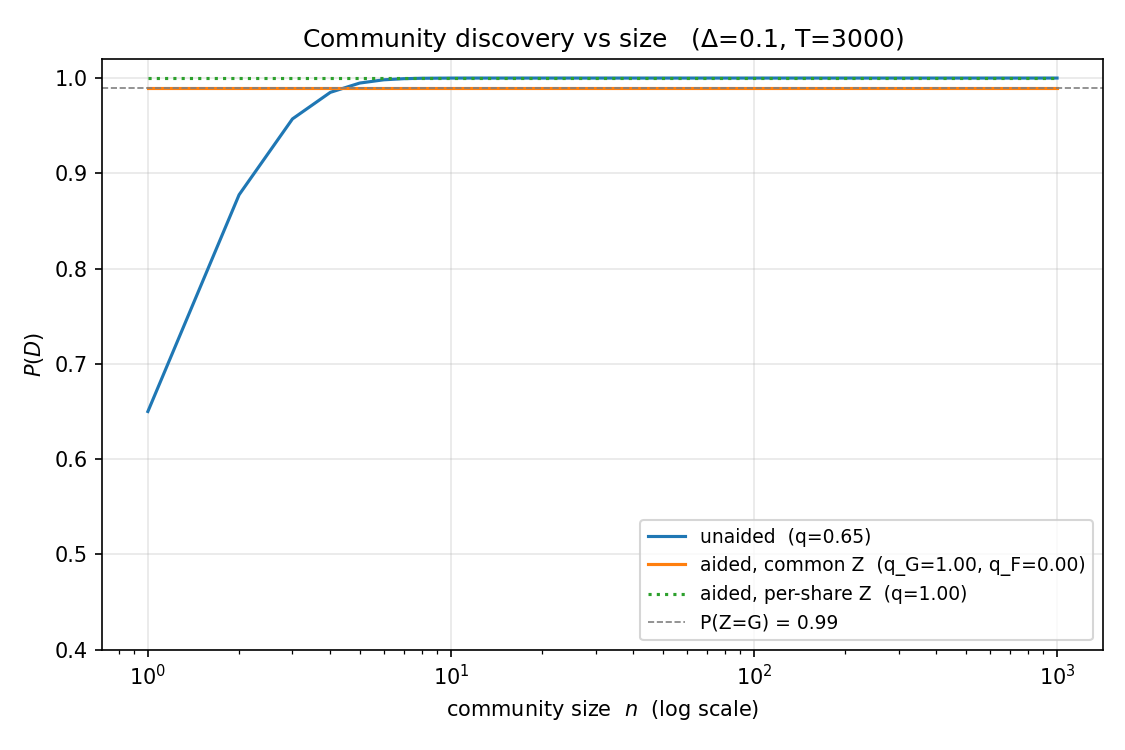
\includegraphics[width=0.75\textwidth]{../results/phase2_es_community_20260610_174604.png}
  \caption{Community discovery probability against community size $n$ for the confused variant at $\Delta = 0.1$, $T = 3000$ (notebook 2). Unaided and per-share-control curves approach $1$; the aided curve with a common $Z$ plateaus at $P(Z = G) = 0.99$: the common failure state cannot be diversified away by adding agents.}
  \label{fig:es-community}
\end{figure}

\paragraph{Corrupted common evidence, not biased sampling.}
The results sharpen what the failure state must \emph{be} for the \S\ref{sec:conj} conjecture to hold at the community level. Suppressing individuals is not enough: the honest variant's $q_F = 0.14$ still leaves $P(D \mid F) = 1 - 0.86^{100} \approx 1$, because a hundred independent gambles virtually guarantee one winner. Community failure requires $q_F \approx 0$ --- every agent's beliefs pushed the same wrong way --- and among the designs above only the confused variant achieves that, by corrupting the evidence map shared by all agents rather than merely biasing which arm gets sampled. First numbers for operationalisation 2 point the same way: a choice nudge at $\varepsilon = 0.1$ gives $0.77$ in $G$ and $0.31$ in $F$ (smoke run at the operating point), and nudges at any strength leave $q_F$ bounded away from zero, since whatever arm is pulled still yields honest data. (The dictatorial nudge $\varepsilon = 1$ is a knife edge: the never-pulled arm $A$ freezes at its flat-prior mean $\tfrac12$, exactly $\delta$ above $B$'s pinned $0.495$, and $\hat q$ sits near $0.48$ on sampling noise.) The conjecture of \S\ref{sec:conj} should therefore be read as a claim about \emph{corrupted common evidence}.

\section{Model conjectures}
\label{sec:conj}

I'm guessing that recommenders and recommendation likelihoods can be defined so that, say,
\[
  P(D_i \mid Z = G) = 0.1, \qquad P(D_i \mid Z = F) = 0.
\]

\ignacio{Pending: pick a concrete recommendation rule $\rho$ that realises these numbers. Candidate from \S\ref{sec:conj}: in $G$, $R$ matches the better arm $A$ with probability $1 - \eta_G$ (tunable); in $F$, $R = B$ with probability $1 - \eta_F$, concentrated at early stages where it bites hardest. Both $\eta_G$ and $\eta_F$ are then sweep parameters to calibrate against the targets $0.1$ and $\approx 0$.}

\michael{$\rho$ doesn't have to realize exactly these numbers. Again, just examples. }

\ignacio{\textbf{Stale numbers below.} The illustrative figures in this section and \S\ref{sec:improve} (unaided $0.05$, aided $0.1$, community $0.994$) predate the flat-prior recalibration of \S\ref{sec:unaided}. At the $\Delta = 0.01$ operating point the unaided baseline is now $q \approx 0.49$ and $P(D) \approx 1 - 6\times10^{-30}$, so the Phase 2 conjectures need restating relative to that baseline --- e.g.\ $P(D_i \mid Z = G)$ somewhat above $0.49$ and $P(D_i \mid Z = F)$ well below it, with the community contrast then driven by the $0.01$ chance of the common failure state rather than by rarity of individual discovery.}

One idea is that in the good state, the recommender is somewhat helpful and often nudges the agent toward the better arm $A$, raising the probability of discovery from $0.05$ to $0.1$.
In the failure condition, the recommender gives misleading $B$ recommendations that prevent success almost surely.
Suppose, for example, that at early stages, when continued sampling of $A$ is important, the recommender often recommends $B$.
If there are enough early $B$ recommendations, the agent won't discover that $A$ is the good arm.

\ignacio{The ``early $B$ bias in $F$'' suggests $\rho$ has time-dependent behaviour ($\eta_F = \eta_F(t)$), not just state-dependent. That is a non-trivial complication for the conditioning step in \S\ref{sec:airec}: the agent's likelihood must depend on $t$ too. Worth deciding before Phase 2 implementation: do we want stationary or non-stationary $\rho$?}

\michael{I was thinking we shouldn't assume that $\rho$ is stationary, that it may exhibit time-dependent behavior.}

\section{Individuals improve, the community gets worse}
\label{sec:improve}

For all $i$, in the aided regime, the probability that $i$ succeeds is
\[
  (0.99)(0.1) + (0.01)(0) = 0.099.
\]
So for each individual the probability of discovery improves from $0.05$ to $0.099$.

The community calculation is different because $Z$ is common across all agents.
Conditional on $Z = G$, the agents still have independent private histories, and each has success probability $0.1$.
So the probability that at least one of the $100$ agents succeeds is
\[
  1 - (1 - 0.1)^{100} \approx 0.99997.
\]
Conditional on $Z = F$, no one succeeds.

So, the aided community discovery probability is
\[
  (0.99)\bigl[1 - (1 - 0.1)^{100}\bigr] + (0.01)(0) \approx 0.98997.
\]
The unaided community success probability is about $0.994$.
So the AI raises every individual's probability of discovery while lowering the community's probability of discovery.

\ignacio{Phase 2 success criterion: a notebook \texttt{2.\ Phase 2 - Aided Bandit.ipynb} that reports $\hat q_{\text{aided}} \approx 0.099$ and $\widehat{P(D)}_{\text{aided}} \approx 0.99$, conditioning explicitly on the recorded $Z$ values per trial. Sweep $\eta_G, \eta_F$ to show the headline result is robust, not knife-edge.}

\section{The mechanism}
\label{sec:mech}

The mechanism is the introduction of dependence from the common AI recommender.
In the unaided regime, some agents get unlucky and abandon $A$, but others continue sampling it.
Their unluckiness is not correlated, so the community benefits from independent variation in payoff histories.

In the aided regime, the agents still have private evidence, but their evidence now includes recommendations generated by the same AI.
In the good condition, this common system helps many agents.
In the rare failure condition, it moves many posteriors in the same wrong direction.
In the aided regime unluckiness becomes correlated.
That is the sense in which this AI recommendation can decrease epistemic diversity.

Finally, note that the model is not a wheel-shaped network with AI as the central node.
The AI does not sample from the arms or generate any payoff history.

\ignacio{Phase 3 (the empirical verification of the mechanism): quantify the correlation explicitly. For each trial compute (a) the cross-agent correlation of $\hat p_A$ trajectories, (b) the conditional correlation given $Z$, and (c) the residual after removing the $Z$-mean. Predict: cross-agent correlation is $\approx 0$ in the unaided regime, $> 0$ in the aided regime, and the gap is entirely attributable to $Z$.}

\section{Next steps}
\label{sec:next}

\begin{enumerate}[leftmargin=*]
  \item Fill in the details of the model and run simulations to confirm the conjectures and effects in sections~\ref{sec:conj} and~\ref{sec:improve}.
  \item Think about how to make the model more interesting.
    For example, we could introduce history-sharing networks together with AI recommendations, and we could model more sophisticated AI recommenders.
\end{enumerate}

\ignacio{Concrete Phase 2 / Phase 3 punch list distilled from the comments above: (1) decide on the discovery definition (\S\ref{sec:bandit}); (2) parameterise $(p_A, p_B, T, \text{prior})$ so unaided $\hat q$ matches the postulated $0.05$ (\S\ref{sec:unaided}); (3) pick the functional form of $\rho$ and whether it is stationary in $t$ (\S\ref{sec:conj}); (4) decide what the agent knows about $Z$ and the per-state likelihoods (\S\ref{sec:airec}); (5) record $Z$ on \texttt{SimulationResult} and report $\widehat{P(D) \mid Z}$ (\S\ref{sec:airec}); (6) verify the mechanism via cross-agent correlations (\S\ref{sec:mech}). Stretch goal (history-sharing networks) is genuinely Phase 4+: the existing \texttt{e\_network\_inequality} codebase will be the reference there.}

\end{document}
